\vspace*{20pt}


\chapter{EK A.1: Haritalar}

\begin{figure}[h!]
\centering{}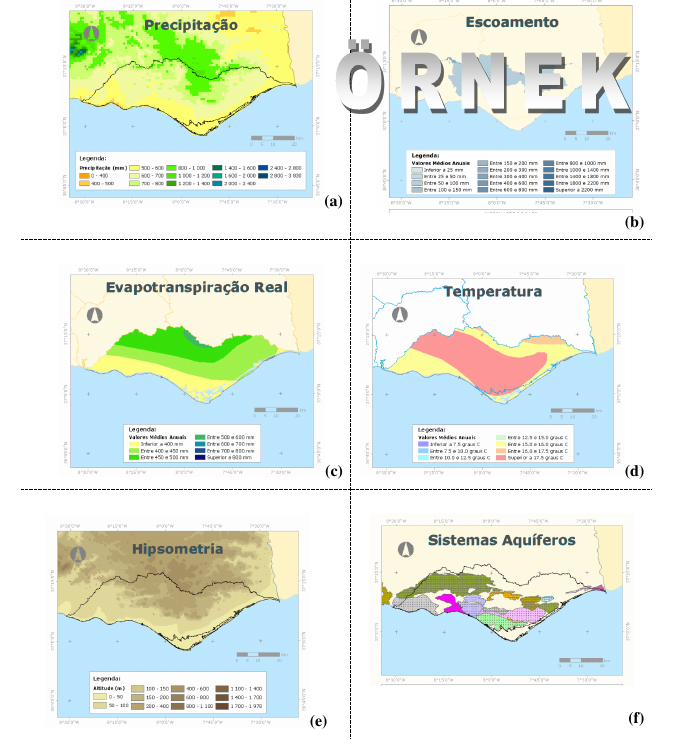
\includegraphics[width=430pt]{fig/haritalar} \caption{\label{fig:6-1}Bölgesel haritalar: (a)Yağış. (b)Akım. (c)Evapotranspirasyon
...}
\end{figure}

\noindent 
\begin{table}
\caption{\label{tableappendix2}Ekler bölümünde çizelge örneği.}

\centering{}%
\begin{tabular}{cccc}
\hline 
Kolon A  & Kolon B  & Kolon C  & Kolon D \tabularnewline
\hline 
Satır A  & Satır A  & Satır A  & Satır A \tabularnewline
Satır B  & Satır B  & Satır B  & Satır B \tabularnewline
Satır C  & Satır C  & Satır C  & Satır C \tabularnewline
\hline 
\end{tabular}
\end{table}

Lorem ipsum dolor sit amet, consectetur adipiscing elit. Sed ac augue
vel dui adipiscing placerat et nec metus. Donec bibendum sodales mollis.
Cras in lacus justo, at vestibulum quam. Sed semper, est sit amet
consectetur ornare, leo est lacinia velit, adipiscing elementum lectus
felis at sem.

\newpage{}

\chapter{EK A.2: Diğer Haritalar}

Lorem ipsum dolor sit amet, consectetur adipiscing elit. Sed ac augue
vel dui adipiscing placerat et nec metus. Donec bibendum sodales mollis.
Cras in lacus justo, at vestibulum quam. Sed semper, est sit amet
consectetur ornare, leo est lacinia velit, adipiscing elementum lectus
felis at sem.

\noindent 
\begin{figure}[h!]
\centering{}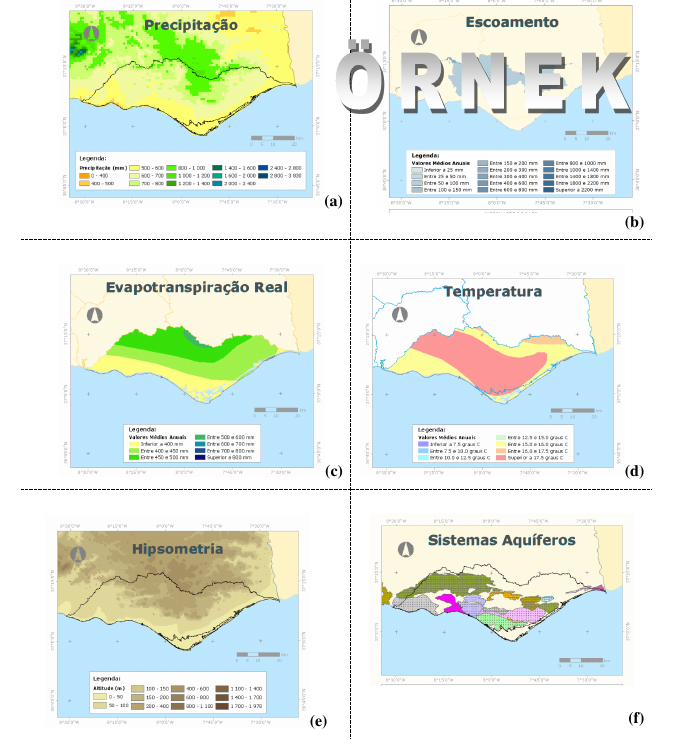
\includegraphics[width=430pt]{fig/haritalar} \caption{\label{fig:6-1-1}Bölgesel haritalar: (a)Yağış. (b)Akım. (c)Evapotranspirasyon
...}
\end{figure}

\noindent 
\begin{table*}[!ht]
\caption{\label{tableappendix2-1}Ekler bölümünde çizelge örneği.}

\centering{}%
\begin{tabular}{cccc}
\hline 
Kolon A & Kolon B & Kolon C & Kolon D\tabularnewline
\hline 
Satır A & Satır A & Satır A & Satır A\tabularnewline
Satır B & Satır B & Satır B & Satır B\tabularnewline
Satır C & Satır C & Satır C & Satır C\tabularnewline
\hline 
\end{tabular}
\end{table*}

Lorem ipsum dolor sit amet, consectetur adipiscing elit. Sed ac augue
vel dui adipiscing placerat et nec metus. Donec bibendum sodales mollis.
Cras in lacus justo, at vestibulum quam. Sed semper, est sit amet
consectetur ornare, leo est lacinia velit, adipiscing elementum lectus
felis at sem.

\newpage{}

\chapter{EK A.3: Diğer Diğer Haritalar}

Lorem ipsum dolor sit amet, consectetur adipiscing elit. Sed ac augue
vel dui adipiscing placerat et nec metus. Donec bibendum sodales mollis.
Cras in lacus justo, at vestibulum quam. Sed semper, est sit amet
consectetur ornare, leo est lacinia velit, adipiscing elementum lectus
felis at sem.

\noindent 
\begin{figure}[h!]
\centering{}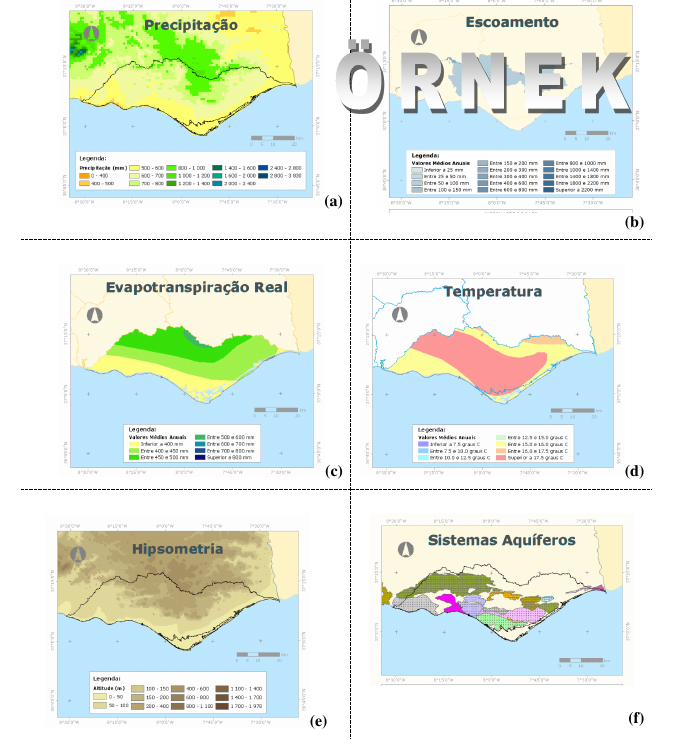
\includegraphics[width=430pt]{fig/haritalar} \caption{\label{fig:6-1-1-1}Bölgesel haritalar: (a)Yağış. (b)Akım. (c)Evapotranspirasyon
...}
\end{figure}

\noindent 
\begin{table*}[!ht]
\caption{\label{tableappendix2-1-1}Ekler bölümünde çizelge örneği.}

\centering{}%
\begin{tabular}{cccc}
\hline 
Kolon A & Kolon B & Kolon C & Kolon D\tabularnewline
\hline 
Satır A & Satır A & Satır A & Satır A\tabularnewline
Satır B & Satır B & Satır B & Satır B\tabularnewline
Satır C & Satır C & Satır C & Satır C\tabularnewline
\hline 
\end{tabular}
\end{table*}

Lorem ipsum dolor sit amet, consectetur adipiscing elit. Sed ac augue
vel dui adipiscing placerat et nec metus. Donec bibendum sodales mollis.
Cras in lacus justo, at vestibulum quam. Sed semper, est sit amet
consectetur ornare, leo est lacinia velit, adipiscing elementum lectus
felis at sem.

\newpage
